\section{Valutazione del modello lineare semplice}\label{i-residui}

$R^{2}$ è un numero compreso tra 0 e 1, ma quanto bene va il mio
modello nel predirre il futuro?

Il modello ottenuto prende in considerazione i dati sui quali è stato
calcolato ed è corretto assumere che, se vengono replicati gli stessi
dati, ci sarà comunque un fattore di diversità tra la stime prodotte e i
dati osservati.

La domanda diventa quindi, quanto i coefficienti stimati sono diversi dai
valori corretti? 

Ad esempio, se si ottiene un $\hat{\beta}_1$ uguale a 0 non si può dire che le \emph{x} e le \emph{y} sono tra loro
indipendenti, ma che il modello lineare non è utile per spiegare \emph{y} utilizzando \emph{x}.

Quindi, quanto è l'errore che otteniamo con il modello ipotizzato?
Quando possiamo dire che $R^2$ è un valore sufficientemente
buono?

Tornando al modello delle vendite, queste sono composte da due
componenti:

\begin{itemize}
\item
  una componente \textbf{sistematica} (deterministica) che viene
  determinata dal modello di regressione e che dipende dalla spesa in
  pubblicità
\item
  una componente \textbf{aleatoria} o erratica, che varia in modo
  stocastico e rappresenta le vendite dovute al caso e non prevedibili.
\end{itemize}

La componente erratica può essere modellata utilizzando una variabile
aleatoria $\epsilon$ con media nulla, il che vuol dire che le
previsioni che risultano maggiori del valore medio sono confrontabili
con quelle che risultano minori.

È inoltre ragionevole assumere che $\epsilon$ sia indipendente sia
da \emph{x} che da \emph{y}, ovvero che tutta la relazione tra \emph{x}
e \emph{y} viene vincolata dalla componente sistematica. Si può
quindi dire che la varianza di $\epsilon$ è costante.

Le ipotesi sul modello diventano quindi

\begin{itemize}
\item
  $e_i$ hanno tutte la stessa distribuzione
\item
  $E(e_i) = 0 \: \forall i$
\item
  per ogni $i\neq j$, $e_i$ è indipendente da $e_j$
\item
  Le varianze degli $e_i$ sono costanti.
\end{itemize}

Con questa definizione si ha che anche \emph{y} è una variabile aleatoria di media $\hat{\beta}_0 + \hat{\beta}_1x$ e varianza $\sigma^2$, questo
perché è una trasformazione lineare di una variabile aleatoria:

dalla teoria delle probabilità si ha che se \textit{Z} è una variabile aleatoria e \textit{a} e \textit{b} sono due costanti, allora:

$$
E(aZ+b) = aE(Z) + b
$$ 

e

$$
\var(aZ+b) = a^2\var(Z)+b
$$

Sempre per quanto riguarda la distribuzione degli errori, sembra essere
ragionevole che la questa sia simmetrica rispetto alla media e che sia più probabile
sbagliare poco, ovvero che segua la distribuzione gaussiana.

$$
\epsilon \sim \mathcal{N}(0,\sigma^2)
$$

Pertanto anche \textit{y} diventa una variabile aleatoria gaussiana.

$$
y \sim \mathcal{N}(\hat{\beta}_0 + \hat{\beta}_1 x, \sigma^2)
$$



\subsection{Valutazione dell'errore di stima su $\hat{\beta}_1$}

Riassumendo:

$$
y = \beta_0 + \beta_1 x + \epsilon \qquad y \sim \mathcal{N}(\beta_0 + \beta_1 x, \sigma^2)
$$
La varianza degli errori $\sigma^2$ viene assunta nota, al fine di semplificare i conti.

La stima di $ \beta_1 $ può quindi essere vista come una determinazione di una variabile casuale. Infatti, se le \textit{y} da cui è calcolata sono il risultato di un esperimento casuale, anche $ \hat{\beta}_1 $ lo è:

$$
\hat{\beta}_1 = \frac{\cov(X,Y)}{\var(X)} = \frac{\sum\limits_{i=1}^n (x_i - \hat{x})(y_i - \bar{y})}{\sum\limits_{i=1}^n (x_i - \bar{x}^2)} = \frac{\sum\limits_{i=1}^n (x_i - \bar{x})y_i}{\sum\limits_{i=1}^n (x_i - \bar{x}^2)} 
$$

Quindi, se le \textit{n} variabili casuali normali $ y_i $ hanno tutte la stessa varianza $ \sigma^2 $ si ha che

$$
\hat{\beta}_1 \sim \mathcal{N}\Bigg(\beta_1 \: , \: \frac{\sigma^2}{\sum_{i=1}^n (x_i - \bar{x})^2}\Bigg)
$$

Questo perché la combinazione lineare di variabili casuali normali è anche essa una variabile casuale normale

$$
a_0 + \sum\limits_{i = 1}^n a_i Z_i \sim \mathcal{N}\bigg(a_0 + \sum\limits_{i=1}^n a_i\mu_i \: , \: \sum\limits_{i=1}^n a_{i}^2 \sigma_{i}^2\bigg)
$$

Da ciò si può osservare che la varianza della stima di $ \hat{\beta}_1  $ coincide con la varianza delle stima delle $ y_i $, scalata per una misura della dispersione delle \textit{x} e che la media di $ \hat{\beta}_1  $ è $ \beta_1 $, ovvero la stima $ \hat{\beta}_1  $ è centrata sul valore vero del parametro, anche se questo è ignoto. Quando questo succede, lo stimatore si dice \textbf{non distorto} o \textbf{corretto}. 

Dal momento che la varianza dello stimatore è influenzata dalla varianza dei campioni utilizzati, conviene cercare di diversificare il più possibile i campioni al fine di avere uno stimatore migliore.

Utilizzando il risultato precedente si può calcolare la distribuzione dell'\textbf{errore di stima}, ovvero $ \hat{\beta}_1  - \beta_1 $, che essendo una trasformazione lineare di una variabile aleatoria\todo{verifcare se l'affermazione è corretta}, risulta essere:

$$
\hat{\beta}_1 - \beta_1 \sim \mathcal{N}\Bigg(0 \: ,\: \frac{\sigma^2}{\sum_{i=1}^n (x_i - \bar{x})^2}\Bigg)
$$

Utilizzando questa nuova variabile aleatoria è possibile andare a calcolare la probabilità che l'errore di stima sia limitato in un certo intervallo, andando prima a trasformare la distribuzione nella normale $ \mathcal{N}(0,1) $ e poi con le tabelle di conversione, andare a calcolare la probabilità effettiva.

\begin{align*}
	P(|\hat{\beta}_1  - \beta_1| < 0.05) &= P\Bigg(\Bigg|\mathcal{N}\bigg(0 \:, \: \frac{\sigma^2}{\sum_{i=1}^n (x_i - \bar{x})^2}\bigg)\Bigg| < 0.05\Bigg) \\
																  &= P\Bigg(\Bigg|\frac{\mathcal{N}\bigg(0\:,\: \frac{\sigma^2}{\sum_{i=1}^n (x_i - \bar{x})^2}\bigg)}{\sqrt{\frac{\sigma^2}{\sum_{i=1}^n (x_i - \bar{x})^2}}}\Bigg| < \frac{0.05}{\sqrt{\frac{\sigma^2}{\sum_{i=1}^n (x_i - \bar{x})^2}}}\Bigg) \\
																  &= P(|\mathcal{N}(0,1)| < 2.342) \text{ (valore recuperato dall'esempio delle slide)} \\
																  &= \Phi(2.342) - \Phi(-2.342) \approx 0.9808\
\end{align*}

In generale un intervallo che contiene il vero valore di un parametro ignoto con probabilità $ 1 - \alpha $ viene chiamato \textbf{intervallo di confidenza $ 1 - \alpha $} e costituisce il modo più semplice di rappresentare la precisione di una stima. Tipicamente come valori di $1 - \alpha $ vengono utilizzati $ 0.5, 0.9, 0.95, 0.99 $.

Più precisamente il procedimento per calcolare un intervallo di confidenza è:

\begin{enumerate}
	\item Fissa un valore per $ 1-\alpha $.
	\item Determina il percentile $ 1 - \alpha/2 $ della normale, ovvero $ P(\mathcal{N}(0,1) \leq z_{1 - \alpha/2}) = 1 - \alpha/2 $.
	\item Si ha quindi che 
	$$
	P\Bigg( \Bigg| (\hat{\beta}_1 - \beta_1) \Bigg/ \sqrt{\frac{\sigma^2}{\sum_{i=1}^n (x_i - \bar{x})^2}}\Bigg| \leq z_{1 - \alpha/2}\Bigg) = 1 - \alpha
	$$
	\item L'intervallo di confidenza di livello $ 1 - \alpha $ risulta quindi essere:
	$$
	\Bigg[ \hat{\beta}_1 - \frac{z_{1-\alpha/2} \cdot \sigma}{\sqrt{\sum_{i=1}^n (x_i - \bar{x})^2}} \: , \: \hat{\beta}_1 + \frac{z_{1-\alpha/2} \cdot \sigma}{\sqrt{\sum_{i=1}^n (x_i - \bar{x})^2}}\Bigg]
	$$
\end{enumerate}

\begin{figure}[htbp]
\centering
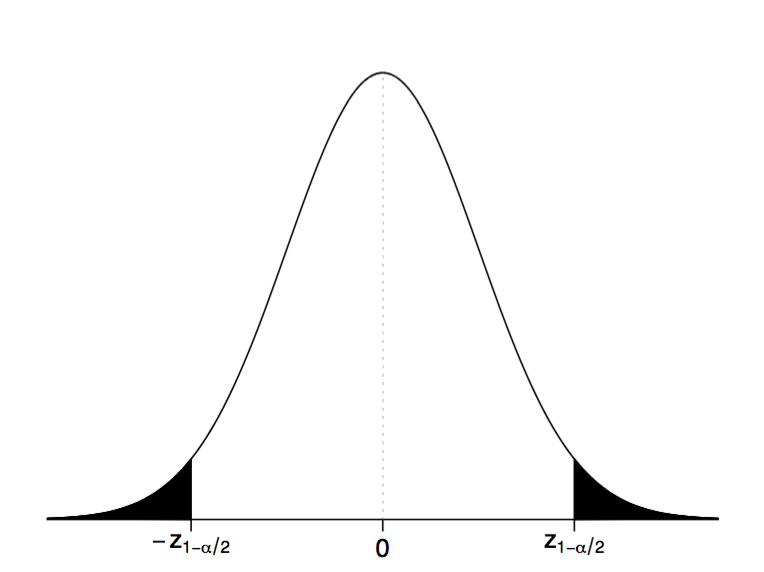
\includegraphics[width = .5\textwidth]{./notes/immagini/l5-fig1-1.png}
\caption{L'area in bianco equivale a $ 1 - \alpha $}
\end{figure}

\subsubsection{Verifica dell'ipotesi}

Un modo alternativo di affrontare la valutazione dell'errore commesso stimando $ \hat{\beta}_1 $ è quello di chiedersi se il modello

$$
y = \beta_0 + \beta_1 x + \epsilon
$$

può essere sostituito dal modello

$$
y = \beta_0 + \epsilon
$$

Si può quindi definire un problema di \textbf{verifica di ipotesi} utilizzando come \textbf{ipotesi nulla} e \textbf{ipotesi alternativa}, rispettivamente:

$$
\begin{cases}
H_0 : \beta_1 = 0 \rightarrow \text{ La spesa in pubblicità influenza le vendite} \\
H_1 : \beta_1 \neq 0  \rightarrow \text{ La spesa in pubblicità non influenza le vendite} 
\end{cases}
$$

\begin{figure}[htbp]
	\centering
	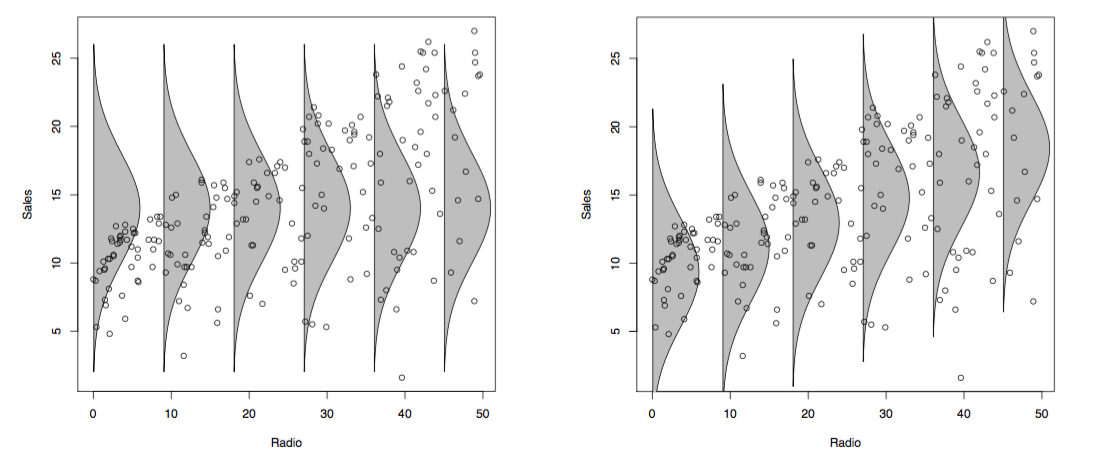
\includegraphics[width = .9\textwidth]{./notes/immagini/l5-fig2-1.png}
	\caption{A sinistra $ H_0 $ e a destra $ H_1 $ per il problema delle vendite.}
\end{figure}


La scelta dell'ipotesi viene effettuata con un \textbf{test statistico} del tipo

$$
-h \leq \frac{\hat{\beta}_1 - 0 }{\sqrt{\frac{\sigma^2}{\sum_{i=1}^n (x_i - \bar{x})^2}}} \leq h
$$

Resta da decidere un valore di soglia per \textit{h} in modo che la probabilità di accettare $ H_0 $ quanto è vera sia 1, ovvero

$$
P\Bigg(-h \leq \frac{\hat{\beta}_1 - 0 }{\sqrt{\frac{\sigma^2}{\sum_{i=1}^n (x_i - \bar{x})^2}}} \leq h \text{ quando }\beta_1 = 0 \Bigg) = 1
$$

ma questo equivale a dire che  \todo{motivare}

$$
P(-h \leq \mathcal{N}(0,1) \leq h) = 1
$$

e questo è vero solo se $ h = + \infty $.
Questo valore di soglia però è inutile, perché si ha che $ H_0 $ viene accettata anche quando è falsa, pertanto ha più senso fissare una soglia che fornisca una probabilità sufficientemente alta, ovvero:

$$
P(\text{accettare } H_0 \text{ quando è vera}) = 1 - \alpha
$$ 

La formulazione diventa quindi

$$
P(-h \leq \mathcal{N}(0,1) \leq h) = 1 - \alpha
$$

ottenendo $ h = z_{1 - \alpha/2} $, dove con $ z_p $ viene indicato il percentile \textit{p}-esimo della normale, ovvero il numero per cui $ \Phi(z_p) = p$.

La procedura per accettare o rifiutare l'ipotesi nulla è quella riportata in figura \ref{fig:ipotesi-1}


\begin{figure}[htbp]
	\centering
	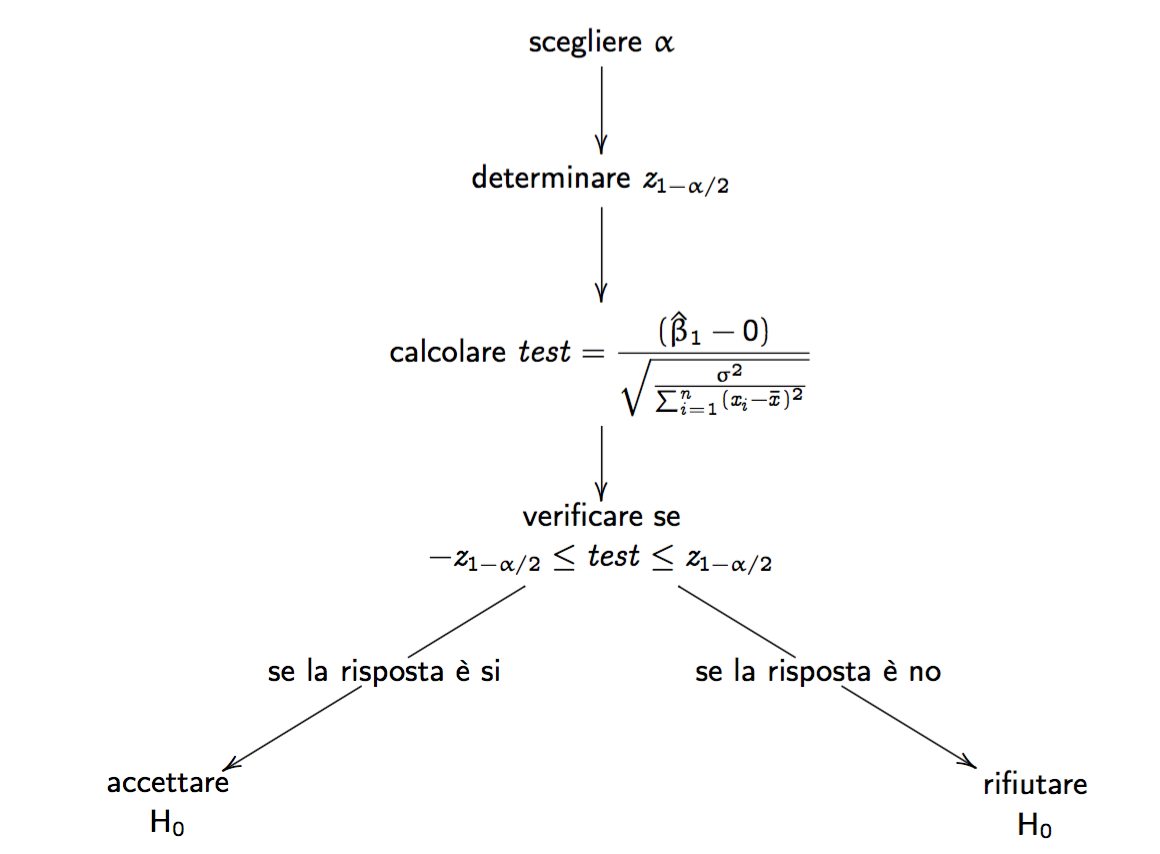
\includegraphics[width = .8\textwidth]{./notes/immagini/l5-fig3-1.png}
	\caption{Procedure per l'accettazione o il rifiuto di $ H_0 $}\label{fig:ipotesi-1}
\end{figure}


